%%%%%%%%%%%%%%%%%%%%%%%%%%%%%%%%%%%%%%%%%%%%%%%%%%%%%%%%%%
%%
%% MARK: Title
%%
%%%%%%%%%%%%%%%%%%%%%%%%%%%%%%%%%%%%%%%%%%%%%%%%%%%%%%%%%%

\chapter*{\S B37.The Diffeology Framework of \hbox{General Covariance}}
\setcounter{footnote}{0}

\vspace{-1em}
%%%%%%%%%%%%%%%%%%%%%%%%%%%%%%%%%%%%%%%%%%%%%%%%%%%%%%%%%%
%%
%% MARK: Abstract
%%
%%%%%%%%%%%%%%%%%%%%%%%%%%%%%%%%%%%%%%%%%%%%%%%%%%%%%%%%%%
\begin{abstract}
  In this lecture%
  \footnote{Talk given at the ``Theory of Gravitation and Variation in Cosmology'' School, CIRM/Luminy, April 12--16, 2021.}
  I will present the principle of general covariance,
  introduced by J.-M. Souriau in the 1970s,
  as the active version of the principle of general relativity.
  I will show how we can include it in the formal diffeology framework.
\end{abstract}

%%%%%%%%%%%%%%%%%%%%%%%%%%%%%%%%%%%%%%%%%%%%%%%%%%%%%%%%%%
%%
%% MARK: The Principle of General Covariance
%%
%%%%%%%%%%%%%%%%%%%%%%%%%%%%%%%%%%%%%%%%%%%%%%%%%%%%%%%%%%
\vspace{-1em}
\section{The principle of general covariance}

Jean-Marie Souriau established his \emph{principle of general covariance} in a few papers,
namely the first two as short notes \cite{Sou70a,Sou70b}:

- {\em Sur le mouvement des particules à spin en relativité générale}.
C. R. Acad. Sci. Paris Sér. A, 271:751–753, 1970.

- {\em Sur le mouvement des particules dans le champ électromagnétique}.
C. R. Acad. Sci. Paris Sér. A, 271:1086–1088, 1970.

Profusely developed and completed in a famous paper \cite{Sou74}:

- {\em Modèle de particule à spin dans le champ électromagnétique et gravitationnel}.
Ann. Inst. Henri Poincaré, XX A, 1974.

The purpose of these papers was to describe the motion of a material medium submitted to the action of a gravitational field,
represented by a pseudo-Riemannian metric $g$,
of signature $(+ -\, -\, -)$,
on a manifold $M$ of dimension $4$,
the \emph{space-time}.

Of course that depends on the nature of the medium:
whether it is a continuous medium or a system of particles,
in the presence of an electromagnetic field or not,
with or without spin, etc.

The motion,
the evolution,
of these systems are described by differential equations,
ordinary or partial differential systems.
In his papers,
Souriau proposes a unique process,
a mechanism,
which gives them all at the same time,
according to the same principle of general covariance,
which can be regarded as the effective \emph{principle of general relativity}.

I should mention that the principle of general covariance is not the only way to find the equations of motion of a material medium in general relativity.
There is obviously the classical variational approach:
the motions are the extremals of some \emph{action functions} defined by a Lagrangian.
I will show later how the two approaches are related.

The point is that it is not apparent if and how the variational approach expresses the principle of general relativity,
but there is no doubt about the principle of general covariance.
We will discuss this.

\begin{Article}{The Physis.}{}
  As we said above,
  let $M$ be a manifold of dimension $4$.
  To describe the motion of a passive material in a gravitational field we shall consider the infinite-dimensional space of all pseudo-Riemannian metrics on $M$.
  Let $\cM$ be this space:
  $$
    \cM = \{ g : \text{pseudo-Riemannian metric} \mid \Sign(g) = (+ -\, -\, -)\}.
  $$
  Now consider the group $\Diff(M)$ of diffeomorphisms of $M$,
  acting by pullback (or pushforward) on $\cM$:
  for all $f \in \Diff(M)$,
  for all $g \in \cM$,
  $$
    f^*(g)_x(v,w) = g_{f(x)}\big(\Der(f)_x(v),\Der(f)_x(w)\big).
  $$
  Now,
  the indifference of the real world with respect to its different representations leads us to regard the gravitational field as equivalently represented by $g$ or by any other metric $g'$ on the same orbit of the group $\Diff(M)$.
  In other words,
  the gravitational field is not $g$ but the orbit
  $$
    \Class(g) = \Diff(M)^*(g).
  $$
  What Souriau proposes is to regard the real world,
  in this case the gravitation,
  as represented not by $\cM$ but by the quotient
  $$
    \bPhi = \cM/\Diff(M).
  $$
  Originally,
  Souriau called the quotient $\cM/\Diff(M)$ the \emph{Hyperspace} and denoted it by $\cH$,
  but in his last unpublished works (``La Grammaire de la Nature'') he changed to \emph{Physis},
  since for him nature expresses itself through this quotient.
  We decide to follow him and denote it by the Greek letter $\bPhi$.
\end{Article}

\begin{figure}[t]
  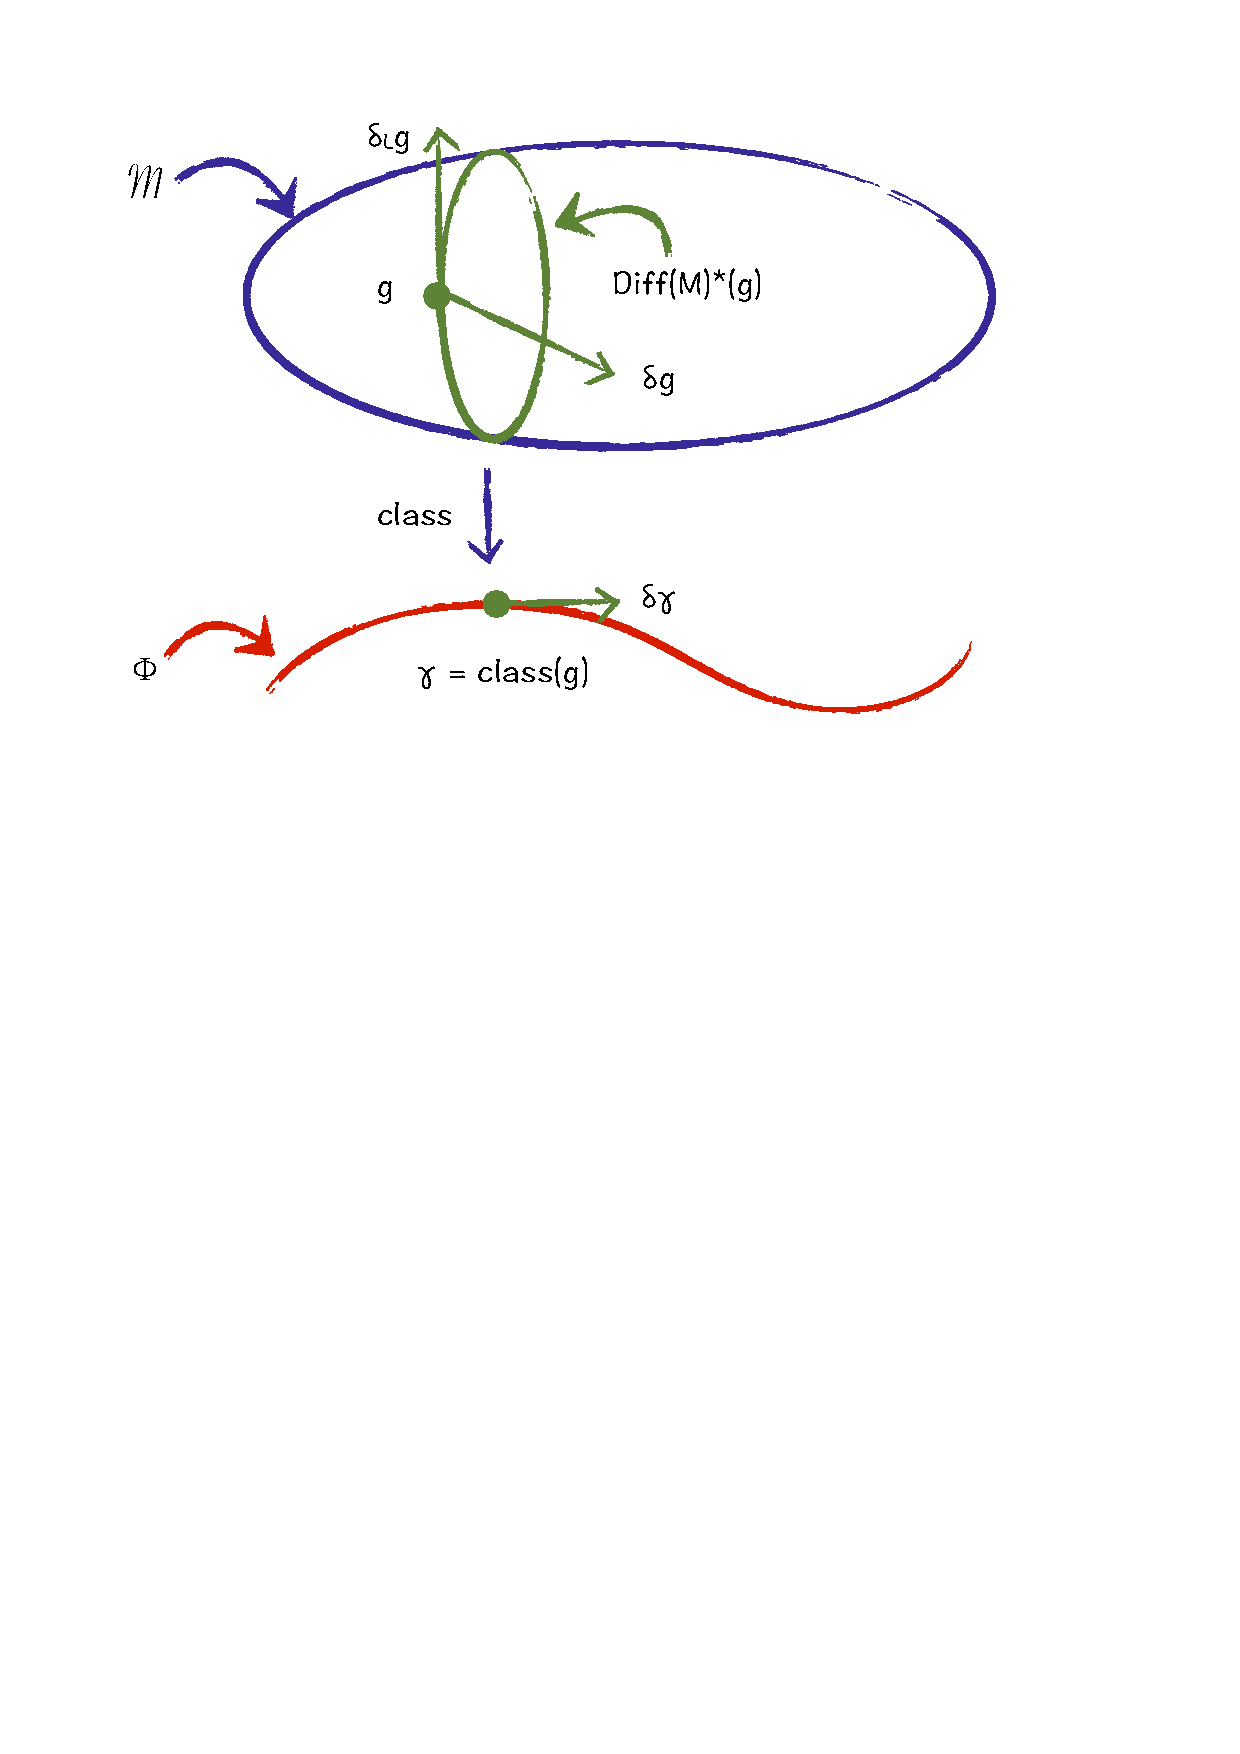
\includegraphics[width=0.65\textwidth]{Figures/fig-Physis.pdf}
  %\vspace{-1.0\baselineskip}
  \caption{The Physis.}
  \label{The-Physis}
\end{figure}

\begin{Article}{The passive matter.}{}
  There are two kinds of evolution of matter in relativity: passive and field-generating.
  The field-generating matter is described by Einstein's equations.
  We may come back to that point later,
  but now we are interested first in the \emph{Passive Equations of Physics},
  as named by Shlomo Sternberg in \cite{Ste12}:
  
  - {\em General Covariance and the Passive Equations of Physics.}
  
  They are defined by the following principle:
  
  \uline{Souriau's principle of general covariance} {\itshape The evolution of matter submitted to a gravitational field is described by a \emph{covector} on the space $\bPhi = \cM/\Diff(M)$.}
  
  Covectors on the space $\bPhi$ are defined by a universal equation we shall establish now.
\end{Article}

\begin{Article}{The universal equation of passive matter.}{}
  We consider a metric
  $$
    g \in \cM
    \quad \text{and} \quad
    \gamma = \Class(g) \in \bPhi.
  $$
  Let us interpret a covector at the point $\gamma$ as a linear functional defined on the variation $\delta\gamma$.
  The point is to understand what $\delta\gamma$ is;
  {\em a priori} it would be a ``tangent vector'' at the point $\gamma$.
  That is,
  a tangent vector $\delta g$ at the point $g$,
  modulo a ``vertical vector'',
  generated by the infinitesimal action of the group $\Diff(M)$.
  
  Thus,
  a linear functional defined on the variation $\delta\gamma$ can be interpreted as a linear functional
  defined on the variations $\delta g$ but vanishing on the vertical vectors.
  
  The variations $\delta g$ are naturally elements of the vector space of covariant symmetric $2$-tensors that we denote by $\cE$:
  $\delta g \in \cE$.
  
  The vertical vectors are generated by differentiation of paths along the orbits of $\Diff(M)$,
  that is,
  $$
    \left.{\partial f_s^*(g) \over \partial s}\right|_{s=0},
    \quad \text{with} \quad
    [s \mapsto f_s] \in \Paths(\Diff(M)),
    \quad \text{and} \quad
    f_0 = \Id_M.
  $$
  Here,
  $\Paths(\Diff(M))$ denotes the smooth paths in $\Diff(M)$ in the sense that $(s,x) \mapsto f_s(x)$ is smooth,
  the variable $s$ being defined on some open neighborhood of $0 \in \RR$.
  
  Then,
  let us define the vector field $\xi$ on $M$ by
  $$
    \xi(x) = \left.{\partial f_s(x) \over \partial s}\right|_{s=0}.
  $$
  Thus,
  the vertical vectors can be written as:
  $$
    \left.{\partial f_s^*(g) \over \partial s}\right|_{s=0} = \left.{\partial \exp(s\xi)^*(g) \over \partial s}\right|_{s=0},
  $$
  that is,
  the \uline{Lie derivative} of the metric $g$ by the vector field $\xi$,
  which we denote by
  $$
    \delta_L g,
    \quad \text{or} \quad \DLie_\xi(g),
    \quad \text{with} \quad
    \delta x = \xi(x).
  $$
  In terms of coordinates,
  the Lie derivative can be written as:
  $$
    \big(\delta_L(g)\big)_{\mu\nu} = \hat\partial_\mu \xi_\nu + \hat\partial_\nu \xi_\mu,
  $$
  where $\hat\partial$ denotes the covariant derivative with respect to the metric $g$.
  The symbol $\hat\partial$ is also denoted by $\nabla$,
  but I prefer the first notation because everything with a hat will refer to covariant differentiation.
  
  In conclusion,
  a covector at the point $\gamma = \Class(g)$ will be represented by a linear functional,
  let us say $\cT$,
  defined on the space $\cE$ of covariant symmetric $2$-tensors $\delta g$,
  and vanishing on the Lie derivative of the metric by any vector field on $M$.
  We can write
  $$
    \Torus^*_\gamma \bPhi = \{ \cT \in \cE^* \mid \cT(\delta_L g) = 0 \text{ for all } \delta x \in \VectorField(M) \},
  $$
  where $\cE^*$ is the dual in some sense that we do not specify now,
  and $\VectorField(M)$ is the space of vector fields on $M$.
  
  In other words,
  the passive motion of matter in a gravitational field $g$ is described by a functional $\cT \in \cE^*$ satisfying the universal equation:
  %
  \begin{equation}\tag{$\clubsuit$}\label{universal-equation}
    \cT(\delta_L g) = 0 \quad \text{for all } \delta x \in \VectorField(M).
  \end{equation}
  %
  Such functionals $\cT$ are called \emph{Eulerian functionals},
  and (\ref{universal-equation}) can be called the \emph{Euler-Souriau equation}.
  We shall understand the choice of vocabulary later.
  
  \uline{Important Note.} Actually,
  for technical reasons and perhaps deeper reasons,
  all the variations considered here,
  all vector fields (which are also variations) will be assumed \emph{compactly supported}.
  We will denote these spaces with a subscript $K$,
  for example $\VectorField_K(M)$,
  $\Diff_K(M)$, etc.
\end{Article}

\begin{Article}{The continuous medium.}{}
  In this framework,
  a continuous medium is described by a continuous distribution of a contravariant symmetric $2$-tensor $\Torus$,
  such that
  $$
    \cT(\delta g) = {1 \over 2} \int_M \Torus^{\mu\nu} \delta g_{\mu\nu} \Vol,
  $$
  where $\Vol$ is the Riemannian volume associated with $g$.
  
  Let us write that $\cT$ is Eulerian:
  \begin{multline*}
    0  =\cT(\delta_L g)
       = {1 \over 2} \int_M \Torus^{\mu\nu} \delta_L g_{\mu\nu} \Vol \\
       = \int_M \Torus^{\mu\nu} \hat\partial_\mu \xi_\nu \Vol
     = \int_M \hat\partial_\mu (\Torus^{\mu\nu} \xi_\nu) \Vol - \int_M \big(\hat\partial_\mu \Torus^{\mu\nu}\big) \xi_\nu \Vol.
  \end{multline*}
  The first term is zero because
  $$
    \hat\partial_\mu (\Torus^{\mu\nu} \xi_\nu) = \hdiv(\eta),
    \quad \text{with} \quad
    \eta^\mu = \sum_\nu \Torus^{\mu\nu} \xi_\nu,
  $$
  and
  $$
    \int_M \hdiv(\eta) \Vol = \int_M \delta_L(\Vol) = \int_M d[\Vol(\eta)] = \int_{\partial M} \Vol(\eta) = 0,
  $$
  since $\eta$ is compactly supported.
  
  Thus,
  it remains from $\cT(\delta_L g) = 0$ the equation
  $$
    \int_M \big(\hat\partial_\mu \Torus^{\mu\nu}\big) \xi_\nu \Vol = 0,
  $$
  for all compactly supported vector fields $\xi$.
  This is equivalent to:
  $$
    \hdiv(\Torus) = 0,
  $$
  which is the conservation equation of a continuous medium in general relativity,
  also called the \emph{Euler equations}.
  This explains the choice of the name ``Eulerian distribution'' for the distributions $\cT$ satisfying condition (\ref{universal-equation}).
\end{Article}

\begin{Article}{The geodesics.}{}
  Now,
  we look for an Eulerian distribution supported by a curve,
  say $t \mapsto x(t)$.
  Thus,
  for all $\delta g$,
  $$
    \cT(\delta g) = {1 \over 2} \int_{-\infty}^{+\infty} \Torus^{\mu\nu} \delta g_{\mu\nu} \, dt.
  $$
  The Eulerian condition becomes:
  \begin{eqnarray*}
    0 & = & \int_{-\infty}^{+\infty} \Torus^{\mu\nu} \hat\partial_\mu\xi_\nu \, dt,
  \end{eqnarray*}
  for all compactly supported vector fields $\xi$.
  For simplicity we assume that the curve exits every compact set.
  
  Multiply the vector field $\xi$ by a real function $\alpha$ that vanishes on the curve;
  we obtain another compactly supported vector field,
  and we get:
  %
  \begin{multline*}
    0 = \int_{-\infty}^{+\infty} \Torus^{\mu\nu} \hat\partial_\mu(\alpha \xi_\nu) \, dt
    = \int_{-\infty}^{+\infty} \Torus^{\mu\nu} \partial_\mu(\alpha) \xi_\nu \, dt + \int_{-\infty}^{+\infty} \alpha \Torus^{\mu\nu} \hat\partial_\mu \xi_\nu \, dt \\
    = \int_{-\infty}^{+\infty} \Torus^{\mu\nu} N_\mu \xi_\nu \, dt + 0 \quad \text{(since $\alpha$ vanishes on the curve)},
  \end{multline*}
  %
  with
  $$
    N = \grad(\alpha) = g^{-1}\!\left({\partial \alpha \over \partial x}\right).
  $$
  Thus,
  $$
    \Torus^{\mu\nu} N_\mu = 0
  $$
  for all vectors $N$ orthogonal to the curve.
  Hence,
  there exists a vector $P$ such that
  $$
    \Torus^{\mu\nu} = P^\mu {dx^\nu \over dt},
  $$
  and since $\Torus^{\mu\nu}$ is symmetric,
  the vector $P$ is parallel to the curve:
  $$
    P \propto {dx \over dt}.
  $$
  Now,
  we substitute this into the universal equation,
  which gives:
  %
  \begin{multline*}
    0 =\int_{-\infty}^{+\infty} P^\mu {dx^\nu \over dt} \hat\partial_\nu\xi_\mu \, dt
    = \int_{-\infty}^{+\infty} P^\mu {\hat\partial \xi_\mu \over \partial x_\nu}{dx^\nu \over dt} \, dt \\
    = \int_{-\infty}^{+\infty} P^\mu {\hat d\,\xi_\mu \over dt} \, dt
    = \int_{-\infty}^{+\infty} {d \over dt}(P^\mu \xi_\mu) \, dt - \int_{-\infty}^{+\infty} {\hat dP^\mu \over dt} \xi_\mu\, dt.
  \end{multline*}
  %
  The first term vanishes since $\xi$ is compactly supported and we have assumed that the curve leaves every compact set.
  It remains:
  $$
    \int_{-\infty}^{+\infty} {\hat dP^\mu \over dt} \xi_\mu \, dt = 0
  $$
  for all $\xi$.
  Therefore,
  $$
    {\hat dP \over dt} = 0.
  $$
  The curve is geodesic and the vector $P$ has constant norm:
  $$
    g(P,P) = P^\mu P_\mu = \text{const}.
  $$
  The value of the constant indicates the type of geodesic of the curve supporting the distribution $\cT$.
  
  Thus,
  we see that the same condition — being Eulerian — encompasses both continuous media and geodesics.
\end{Article}

\begin{Article}{Others\dots}{}
  I will not develop more examples in this short note;
  you can see \cite{Sou74} and also \cite{Ste12}.
  
  Let us say that the universal equation above (\ref{universal-equation}) gives all kinds of passive equations of motion
  for almost everything we can think of:
  strings,
  charged particles in an electromagnetic field (we should add the electromagnetic potential $A$ to the metric and the gauge transformation group),
  charged particles with spin in gravitational and electromagnetic fields, and so on.
  
  We can also find the laws of \uline{reflection and diffraction of dust in a gravitational field}
  along a discontinuity of the metric,
  by adapting the Eulerian condition to the group of diffeomorphisms preserving the locus of the singularity \cite{PIZ19}.
\end{Article}

\begin{Article}{Covariance and variation.}{}
  As we said,
  the calculus of variations is the classical way to obtain the equations of motion of passive matter in general relativity.
  
  We have an action $A$ depending on some fields $\sigma$ in some given geometry $g$.
  This action is the integral of some Lagrangian function which depends on the specific problem.
  For example: for geodesics, $\sigma$ is a curve and $A$ is the length of the curve.
  The equations of motion are the critical points of $\sigma$ satisfying the equation:
  $$
    {\partial A \over \partial \sigma}(\delta \sigma) = 0.
  $$
  Now consider the geometry as part of the action $A$,
  that is,
  the action is a function of $g$ and $\sigma$.
  Assume that there is a group $\bmG$ that acts on the space $\cM$ of geometries and on the space $\Sigma$ of fields $\sigma$ such that:
  \begin{enumerate}
    \item The action is invariant under the action of $\bmG$ acting diagonally on $\cM \times \Sigma$.
    \item The group $\bmG$ acts transitively on the space of fields.
  \end{enumerate}
  Thus,
  the invariance of $A$ gives the identity
  $$
    {\partial A \over \partial g}(\delta_L g) + {\partial A \over \partial \sigma}(\delta_L \sigma) = 0,
  $$
  where $\delta_L$ denotes a derivation along the $1$-parameter subgroups of $\bmG$.
  Then,
  since $\bmG$ acts transitively on the space $\Sigma$,
  the identity above becomes
  $$
    {\partial A \over \partial g}(\delta_L g) + {\partial A \over \partial \sigma}(\delta \sigma) = 0,
  $$
  for all $\delta \sigma$.
  Thus,
  if $\sigma$ is a critical point of $A$ for some value of the geometry $g$,
  then the covector
  $$
    \cT = {\partial A \over \partial g}
    \quad \text{satisfies} \quad
    \cT(\delta_L g) = 0,
  $$
  for all $\delta \sigma$.
  The covector $\cT$ is Eulerian.
  
  Conversely,
  if the covector $\cT$ is Eulerian for a value $\sigma$ in some geometry $g$,
  then $\sigma$ is a critical point of the action $A$.
  
  The two principles indeed give the same solutions;
  they mirror each other.
  
  However,
  in the absence of a Lagrangian action,
  the principle of general covariance generalizes the \emph{Principle of Least Action}.
  
  It has the virtue,
  in addition to generalizing the construction of the passive equations of physics,
  of \emph{changing the paradigm} of physics,
  from a metaphysical principle of least action to a geometrical invariance constraint,
  which is more tangible.
  
  \uline{Remark.} One should note, however, that the principle of general covariance does not find the irrational geodesics on the $2$-torus,
  since the integral $\cT(\delta g) = {1 \over 2} \int_{-\infty}^{+\infty} P^\mu {dx^\nu \over dt} \delta g_{\mu\nu} \, dt$ does not converge for all $\delta g$,
  except on closed geodesics.
\end{Article}

\begin{Article}{The principle of general relativity.}{}
  It is time to discuss the relationship between Einstein's \emph{Principle of General Relativity} and Souriau's \emph{principle of general covariance}.
  Usually the principle of general relativity is stated as follows:
  
  - {\em Physical laws are the same in all reference frames — inertial or non-inertial.}
  
  This statement is vague enough to have made Vladimir Fock say:
  ``There is no general relativity, only a theory of gravitation.''
  Indeed,
  what are the laws of physics,
  and how do you express them?
  What does it mean to be the same in all frames?
  Same according to what?
  Clearly, this is unsatisfactory.
  
  There is another formulation that can be found in the literature:
  
  - {\em The equations of physics are covariant under changes of coordinates.}
  
  Still unsatisfactory;
  too many terms are not well defined.
  
  On the other hand,
  the principle of general covariance is clear and unambiguous:
  the objects are well defined and the universal equation (\ref{universal-equation}) is unique and clear.
  
  There is another difference between the usual statement of the principle of general relativity and the principle of general covariance:
  
  The principle of general relativity is a passive way of referring to nature.
  It concerns the various means of describing parts of the world,
  through the various charts used to refer to objects.
  
  The principle of general covariance is an active approach in the sense that the group of diffeomorphisms \emph{acts} effectively on the geometries.
  The statement is not vague and says precisely:
  in general relativity,
  the objects of nature are covectors of the Physis,
  the quotient of the geometries by the group of diffeomorphisms of space-time.
\end{Article}

%%%%%%%%%%%%%%%%%%%%%%%%%%%%%%%%%%%%%%%%%%%%%%%%%%%%%%%%%%
%%
%% MARK: The Diffeology Framework
%%
%%%%%%%%%%%%%%%%%%%%%%%%%%%%%%%%%%%%%%%%%%%%%%%%%%%%%%%%%%
\section{The Diffeology framework}

\begin{Article}{The compact diffeology on $\cM$.}{}
  Let $\cM$ be the set of pseudo-Rie\-man\-nian metrics on a manifold $M$,
  of signature $(+ -\, -\, -)$.
  It is a subset of smooth maps from $M$ to the covariant $2$-tensor bundle $S_2(M)$ over $M$;
  these are smooth sections.
  %
  Since $M$ and $S_2(M)$ are manifolds,
  $\Cinfty(M,S_2(M))$ is equipped with the functional diffeology,
  and $\cM \subset \Cinfty(M,S_2(M))$ will be equipped with the subset diffeology.
  
  Now, we will equip $\cM$ with a sub-diffeology of the functional diffeology:
  
  \uline{Definition.} {\itshape A smooth parametrization $r \mapsto g_r$ in $\cM$,
  defined on some Euclidean domain $U$,
  is a plot of the \emph{compact diffeology} if:
  for all $r \in U$ there exists an open neighborhood $V \subset U$ of $r$ and a compact $K \subset M$ such that:
  $$
    \forall r' \in V,\ \forall x \in M \setminus K,\quad g_{r'}(x) = g_{r}(x).
  $$}
  Indeed,
  constant parametrizations satisfy this condition.
  The condition is obviously local.
  By composition with a smooth parametrization $F$ in $U$,
  the neighborhood $V$ becomes $F^{-1}(U)$ for the same compact $K$.
  
  \uline{Note.} Let $r \mapsto g_r$ be a plot of the compact diffeology.
  Since $M$ and $S_2(M)$ are manifolds,
  the variation
  $$
    {\partial g_r(x) \over \partial r}(\delta r)
  $$
  is a well-defined symmetric $2$-tensor on $M$,
  and is compactly supported.
  Indeed,
  $$
    {\partial g_r(x) \over \partial r}(\delta r) = \lim_{s \to 0} {1 \over s} \big[g_{r + s \delta r}(x) - g_r(x)\big].
  $$
  For $\epsilon \in \RR$ sufficiently small,
  for all $|s| < \epsilon$,
  $r + s \delta r$ will be contained in a ball contained in the neighborhood $V$ for which $g_{r'}(x) = g_r(x)$ outside some compact $K$.
  Thus,
  as $s \to 0$,
  $g_{r + s \delta r}(x) - g_r(x) = 0$ outside $K$,
  so the variation of $g_r$ is compactly supported.
\end{Article}

\begin{Article}{Pushing forward pointed differential forms.}{}
  In the chapter ``On Riemannian metric in diffeology'' we have seen the definition of pointed differential forms.
  Now,
  the general criterion for pushing forward differential forms can be adapted here.
  There are two cases:
  the general % \pagebreak %% PIZ finetunning
  %
  case of a subduction and the special case of a \emph{local subduction} \cite[\textsection\,2.16]{PIZ13}.
  
  Recall that a subduction $\pi \colon Y \to X$ is said to be a local subduction if for all plots $P \colon U \to X$,
  for all $r \in U$ and all $y \in \pi^{-1}(x)$,
  $x = P(r)$,
  there exists a local lift $Q$ in $Y$,
  that is,
  $\pi \circ Q = P \restriction \Domain(Q)$,
  such that $Q(r) = y$.
  
  In particular,
  projections onto quotients by actions of groups of diffeomorphisms are local subductions.
  
  Let us come back to the general case.
  Let $\alpha_y$ be a pointed $k$-form.
  
  \uline{Proposition 1.} {\itshape There exists a pointed $k$-form $\beta_x$,
  with $x = \pi(y)$,
  such that $\alpha_y = \pi^*(\beta_x)$ if and only if for all $y' \in \pi^{-1}(x)$ there exists a pointed form $\alpha_{y'}$ such that:
  for all pairs of plots $P'$ and $P''$,
  pointed in the fiber $\pi^{-1}(x)$,
  with $\pi \circ P' = \pi \circ P''$,
  $\alpha_{y'}(P') = \alpha_{y''}(P'')$ where $y' = P'(0)$ and $y'' = P''(0)$.}
  
  If $X = Y/G$,
  where $G$ is a diffeological group acting on $Y$ by diffeomorphisms,
  the situation is simpler because $\pi$ is a local subduction.
  In this case,
  we have:
  
  \uline{Proposition 2.} {\itshape In the case $X = Y/G$,
  there exists a pointed $k$-form $\beta_x$,
  with $x = \pi(y)$,
  such that $\alpha_y = \pi^*(\beta_x)$ if and only if for all plots $P'$ and $P''$ pointed at $y$,
  $\pi \circ P' = \pi \circ P''$ implies $\alpha_y(P') = \alpha_y(P'').$}
\end{Article}

\begin{Article}{Proposition: The Physis.}{}
  Consider the group of diffeomorphisms with compact support $\Diff_K(M)$,
  that is,
  the diffeomorphisms of $M$ that are the identity outside a compact set.
  
  The group $\Diff_K(M)$ acts on the set $\cM$ of pseudo-Riemannian metrics on $M$ by pullback:
  $$
    f^* \colon \cM \to \cM,
    \quad \text{with} \quad
    f^*(g)_x(v,w) = g_{f(x)}\big(\Der(f)_x(v),\Der(f)_x(w)\big).
  $$
  Equip $\cM$ with the compact diffeology.
  Let $\bPhi$ be the quotient space:
  $$
    \bPhi = \cM/\Diff_K(M).
  $$
  
  \uline{Claim 1.} {\itshape The group $\Diff_K(M)$ acts on $\cM$ by diffeomorphisms.
  Therefore,
  the projection $\Class \colon \cM \to \bPhi$ is a local subduction.}
  
  Now,
  let us equip the group $\Diff_K(M)$ with the \emph{compact functional diffeology}.
  A parametrization $P \colon r \mapsto f_r$,
  defined on $U$,
  in $\Diff_K(M)$ will be a plot if it is a plot for the functional diffeology and if:
  
  \uline{Definition.} {\itshape For all $r \in U$ there exists an open neighborhood $V$ of $r$ and a compact $K \subset M$ such that:
  for all $r' \in V$,
  $f_{r'}$ is the identity outside $K$.}
  
  \uline{Claim 2.} {\itshape Equipped with the compact functional diffeology,
  the group $\Diff_K(M)$ acts smoothly on $\cM$.
  That is,
  the map $f \mapsto f^*$ is smooth.}
\end{Article}

\begin{proof}
  First of all,
  $f^*$ is bijective;
  its inverse is $(f^{-1})^*$.
  Now, let $P \colon r \mapsto g_r$ be a plot of the compact diffeology.
  Let $r \in \Domain(P)$.
  There exists an open neighborhood $V$ of $r$ and a compact $K \subset M$ such that:
  for all $r' \in V$,
  for all $x \in M \setminus K$,
  $g_{r'}(x) = g_r(x)$.
  Thus,
  for all $r' \in V$,
  for all $x \in M \setminus f^{-1}(K)$,
  $f^*(g_{r'})(x) = f^*(g_r)(x)$.
  The parametrization $f^* \circ P$ is then a plot of $\cM$.
  The same holds for $(f^{-1})^*$.
  Therefore,
  $f^*$ is a diffeomorphism of $\cM$.
  
  Let us prove now that the action map
  $$
    \Diff_K(M) \times \cM \to \cM,
    \quad (f,g) \mapsto f^*(g),
  $$
  is smooth.
  Let $r \mapsto (f_r, g_r)$ be a plot defined on some $U$.
  Let us show that $r \mapsto f_r^*(g_r)$ is smooth for the compact diffeology.
  It is already smooth for the functional diffeology;
  all that remains is the question of compact support.
  
  Let $r \in U$.
  There exists an open neighborhood $V$ of $r$ and two compacts $K, K' \subset M$ such that,
  for all $r' \in V$,
  for all $x \notin K$, $g_{r'}(x) = g_r(x)$,
  and for all $x \notin K'$, $f_{r'}(x) = f_r(x) = x$.
  We need to compare $f_r^*(g_r)(x)$ and $f_{r'}^*(g_{r'})(x)$.
  For all $r' \in V$ and $x \notin K'$,
  $f_{r'}(x) = f_r(x) = x$,
  so $f_{r'}^*(g_{r'})(x) = g_{r'}(x)$ and $f_r^*(g_r)(x) = g_r(x)$.
  Now, for all $x \notin K$,
  $g_{r'}(x) = g_r(x)$.
  Thus,
  if $r' \in V$ and $x \notin K'' = K \cup K'$,
  we have $f_r^*(g_r)(x) = f_{r'}^*(g_{r'})(x)$.
  Since $K''$ is compact,
  $r \mapsto f_r^*(g_r)$ is a plot in $\cM$ and the action is smooth.
\end{proof}

\begin{Article}{Pointed differential forms on the Physis.}{}
  Let $\cT$ be a real smooth bounded linear operator defined on the subspace $\cE \subset S_2(M)$ of symmetric covariant $2$-tensors with compact support.
  That is,
  
  \begin{enumerate}
    \item $\cT \colon \cE \to \RR$,
    and $\cT(a \epsilon + a'\epsilon') = a \cT(\epsilon) + a'\cT(\epsilon')$,
    for all $a, a' \in \RR$ and $\epsilon, \epsilon' \in \cE$.
    \item $\cT \in \Cinfty(\cE, \RR)$.
    \item For all $\epsilon \in \cE$,
    there exists a constant $c$ such that:
    $|\cT(\epsilon)| \leq c \|\epsilon\|$ for some norm on the space $\cE$.
  \end{enumerate}
  
  Now,
  for all $n$-plots $r \mapsto g_r$ pointed at $g = g_0$,
  define $\tau_g$ by
  $$
    \tau_g(r\mapsto g_r)(v) = \cT\!\left(\left.{\partial g_r \over \partial r}\right|_{r=0}(v)\right)
    \quad \text{for all } v \in \RR^n.
  $$
  We know that since $r \mapsto g_r$ is a plot for the compact diffeology,
  $$
    {\partial g_r \over \partial r}(\delta r) \in \cE.
  $$
  Thus,
  $$
    \cT\!\left({\partial g_r \over \partial r}(\delta r)\right)
  $$
  is well defined.
  So is $\tau_g(r\mapsto g_r)$,
  which belongs to $\Lambda^1(\RR^n)$.
  
  \uline{Claim 2.} {\itshape The process $\tau_g$ is a differential $1$-form pointed at $g$.}
  
  Now,
  
  \uline{Claim 3.} {\itshape Consider two plots $P \colon r \mapsto g_r$ and $P' \colon r \mapsto g'_r$ pointed at $g = g_0 = g'_0$.
  Assume $\Class(g_r) = \Class(g'_r)$ such that there exists a plot $r \mapsto f_r$ with $g'_r = f_r^*(g_r)$ and $f_0 = \Id_M$.
  Then,
  $\tau_g(r\mapsto g_r) = \tau_g(r\mapsto g'_r)$ if and only if
  $$
    \cT(\delta_L g) = 0
  $$
  for all compactly supported vector fields $\delta x$.
  
  In that case,
  there indeed exists a linear $1$-form $\sigma$ pointed at $\gamma = \Class(g)$ such that $\tau_g = \Class^*(\sigma)$.}
  
  Thus,
  Eulerian distributions indeed represent special $1$-forms pointed somewhere in the quotient $\bPhi$.
  
  \Note It remains to be seen what the obstacles are to the existence of a smooth map $r \mapsto f_r$ such that $\Class \circ g'_r = \Class \circ g_r$ in general.
  Probably,
  the subspace of pseudo-Riemannian metrics without isometries with compact support forms a principal diffeological fiber bundle over its quotient by $\Diff_K(M)$,
  and therefore such a smooth map $r \mapsto f_r$ always exists in this situation.
\end{Article}

\begin{proof}
  Consider $\tau_g$.
  Let $s \mapsto r \mapsto g_r$,
  where $s \mapsto r$ is a plot in $\RR^n$ pointed at $0$.
  Then,
  \begin{eqnarray*}
    \tau_g(s\mapsto g_r)(w) & = & \cT\!\left(\left.{\partial g_r \over \partial s}\right|_{s=0}(w)\right) \\
    & = & \cT\!\left(\left.{\partial g_r \over \partial r}\right|_{r=0}\!\left(\left.{\partial r \over \partial s}\right|_{s=0}(w)\right)\right).
  \end{eqnarray*}
  On the other hand,
  \begin{eqnarray*}
    [s \mapsto r]^*\big(\tau_g(r\mapsto g_r)\big)(w) & = & \tau_g(r\mapsto g_r)\!\left(\left.{\partial r \over \partial s}\right|_{s=0}(w)\right) \\
    & = & \cT\!\left(\left.{\partial g_r \over \partial r}\right|_{r=0}\!\left(\left.{\partial r \over \partial s}\right|_{s=0}(w)\right)\right).
  \end{eqnarray*}
  Thus,
  $\tau_g(s \mapsto r \mapsto g_r) = [s \mapsto r]^*\big(\tau_g(r\mapsto g_r)\big)$.
  Therefore,
  $\tau_g$ is a differential $1$-form pointed at $g$.
  
  Next,
  let $g'_r = f_r^*(g_r)$.
  We have
  \begin{eqnarray*}
    \left.{\partial g'_r \over \partial r}\right|_{r=0}(v) & = & \left.{\partial f_r^*(g_r) \over \partial r}\right|_{r=0}(v) \\
    & = &  \left.{\partial f_r^*(g) \over \partial r}\right|_{r=0}(v) + \left.{\partial g_r \over \partial r}\right|_{r=0}(v).
  \end{eqnarray*}
  Now let $\pphi_s(x) = f_{sv}(x)$,
  with $s$ real.
  Then,
  $$
    \left.{\partial f_r^*(g) \over \partial r}\right|_{r=0}(v) = \left.{\partial \pphi_s^*(g) \over \partial s}\right|_{s=0},
  $$
  and defining the vector field $\xi$ by
  $$
    \xi(x) = \left.{\partial \pphi_s(x) \over \partial s}\right|_{s=0},
  $$
  we obtain:
  $$
    \left.{\partial f_r^*(g) \over \partial r}\right|_{r=0}(v) = \delta_L g
    \quad \text{with} \quad
    \delta x = \xi(x).
  $$
  Thus,
  $$
    \left.{\partial g'_r \over \partial r}\right|_{r=0}(v) = \left.{\partial g_r \over \partial r}\right|_{r=0}(v) + \delta_L g.
  $$
  Hence:
  $$
    \cT(\delta g') = \cT(\delta g) + \cT(\delta_L g),
  $$
  where
  $$
    \delta g = \left.{\partial g_r \over \partial r}\right|_{r=0}(v).
  $$
  Therefore,
  the $1$-form $\tau_g$ pointed at $g$ descends to the quotient if $\cT$ is Eulerian.
\end{proof}

\vfill
\centerline{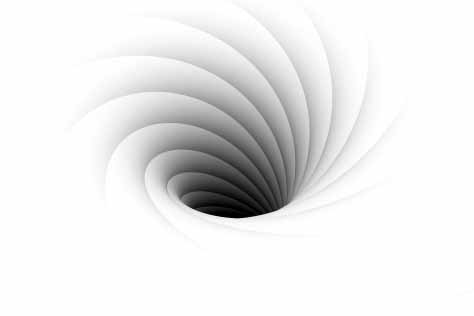
\includegraphics[width=1\textwidth]{Figures/BlackHole.jpg}}
\vspace{50pt}
